% Template for Cogsci submission with R Markdown

% Stuff changed from original Markdown PLOS Template
\documentclass[10pt, letterpaper]{article}

\usepackage{cogsci}
\usepackage{pslatex}
\usepackage{float}
\usepackage{caption}

% amsmath package, useful for mathematical formulas
\usepackage{amsmath}

% amssymb package, useful for mathematical symbols
\usepackage{amssymb}

% hyperref package, useful for hyperlinks
\usepackage{hyperref}

% graphicx package, useful for including eps and pdf graphics
% include graphics with the command \includegraphics
\usepackage{graphicx}

% Sweave(-like)
\usepackage{fancyvrb}
\DefineVerbatimEnvironment{Sinput}{Verbatim}{fontshape=sl}
\DefineVerbatimEnvironment{Soutput}{Verbatim}{}
\DefineVerbatimEnvironment{Scode}{Verbatim}{fontshape=sl}
\newenvironment{Schunk}{}{}
\DefineVerbatimEnvironment{Code}{Verbatim}{}
\DefineVerbatimEnvironment{CodeInput}{Verbatim}{fontshape=sl}
\DefineVerbatimEnvironment{CodeOutput}{Verbatim}{}
\newenvironment{CodeChunk}{}{}

% cite package, to clean up citations in the main text. Do not remove.
\usepackage{cite}

\usepackage{color}

% Use doublespacing - comment out for single spacing
%\usepackage{setspace}
%\doublespacing


% % Text layout
% \topmargin 0.0cm
% \oddsidemargin 0.5cm
% \evensidemargin 0.5cm
% \textwidth 16cm
% \textheight 21cm

\title{Language use shapes cultural biases: Large scale evidence from gender}


\author{{\large \bf Molly Lewis} \\ \texttt{mollyllewis@gmail.com} \\ Department of Psychology  \\ University of Wisconsin-Madison \And {\large \bf Gary Lupyan} \\ \texttt{lupyan@wisc.edu} \\ Department of Psychology  \\ University of Wisconsin-Madison}

\begin{document}

\maketitle

\begin{abstract}
The abstract.

\textbf{Keywords:}
IAT, cultural biases, gender, linguistic relativity.
\end{abstract}

\section{Introduction}\label{introduction}

The language we use to communicate a message shapes how our listener
interprets that message (Fausey \& Boroditsky, 2010; Loftus \& Palmer,
1996; Tversky \& Kahneman, 1981). A listener, for example, is more
likely to infer that a person is at fault if the event is described
actively (e.g., ``she ignited the napkin''), as opposed to passively
(e.g., ``the napkin ignited''). The formative power of language is
perhaps most potent in shaping meanings that necessarily must be learned
from others: cultural meanings. In the present paper, we consider one
type of cultural meaning---gender---and examine the extent to which
differences in languge use may lead to cross-cultural differences in
understandings of gender.

The gender domain is a useful case study of the relationship between
language and thought for a number of reasons. First, there is reason to
think that abstract domains, like gender, may be more subject to the
influence of language relative to more perceptually grounded domains
(Boroditsky, 2001). Second, many langauges encode gender explicitly in
their grammar. Third, there is a large body of evidence suggesting that
language plays a key role in transmitting social knowledge to children
(e.g., Master, Markman, \& Dweck, 2012). And, foruth, gender norms are
highly variable across cultures and have clear and important social
implications.

For our purposes, we define the hypothesis space of possible
relationships between language and gender biases with two broad
extremes: (1) language reflects a pre-existing gender bias in its
speakers (\emph{language-as-reflection hypothesis}); (2) language
causally influences gender biases (\emph{language-as-causal
hypothesis}). We assume that the language-as-reflection hypothesis is
true to some extent; the way we talk about gender almost certainly
reflects how we think about gender. If, for example, you think nurses
are most commonly women, you are likely to use a female pronoun to refer
to a generic nurse. Our goal here is to understand the extent to which
language may also exert a causal influence on conceptualizations of
gender.

In particular, we explore two possible mechanisms by which the way we
speak may influence notions of
gender.\footnote{These mechanisms are what Whorf (1945) refers to as phenotypes (overt) and cryptotypes (covert).}
The first is through the overt grammatical marking of gender on nouns,
which are obligatory in roughly one quarter of languages (e.g., in
Spanish, ``nina'' (girl) and ``enfermera'' (nurse) both take the gender
marker \emph{-a} to indicate grammatical femininity; Corbett, 1991).
Because grammatical gender has a natural link to the real world,
speakers may assume that grammatical markers are meaningful even when
applied to inanimate objects that do not have a biological sex. In
addition, the mere presence of obligatory marking of grammatical gender
may promote bias by making the dimension of gender more salient to
speakers.

A second route by which language may shape psychological gender is
through the distribution of words in use: Words that tend to occur in
similar contexts in language may lead speakers to assume---either
implicitly or explicitly---that they have similar meanings. For example,
statistically, the word ``nurse'' occurs in many of the same contexts as
the pronoun ``her,'' providing an implicit link between these two
concepts that may lead to a bias to assume that nurses are female. This
second route may be particularly influential because the bias is encoded
in language in a way that is more implicit than grammatical markers of
gender.

There is an existing body of experimental work that points to a link
between language and psychological gender bias in both adults (e.g.,
Phillips \& Boroditsky, 2003) and children (e.g., Sera, Berge, \&
Castillo Pintado, 1994). For example, Phillips and Boroditsky (2003)
asked Spanish-English and German-English adult bilinguals to make
similarity judgements between pairs of pictures depicting an object with
a natural gender (e.g., a bride) and one without (e.g., a toaster). They
found that participants rated pairs as more similar when the pictures
matched in grammatical gender in their native language. While these
types of studies provide suggestive evidence for a causal link between
language and psychological gender bias, they are limited by the fact
that they typically only compare speakers of 2-3 different languages and
measure bias in a way that is subject to demand characteristics.

In what follows, we ask whether the way gender is encoded linguistically
across 31 different languages predicts cross-cultural variability in the
bias to associate men with careers and women with family. We begin in
Study 1 by describing cross-cultural variability in psychological gender
biases using an implicit measure. In Study 2, we use machine learning
methods to describe lexical semantics, and ask whether variability in
lexical semantics predicts variability in psychological gender bias. In
Study 3, we ask whether the presence of grammatical gender in a language
predicts gender bias. Together, our data suggest that language likely
plays a causal role in shaping culturally-specific notions of gender.

\section{Study 1: Cross-cultural variability in gender
bias}\label{study-1-cross-cultural-variability-in-gender-bias}

In Study 1, we describe cross-cultural variability in psychological
gender bias. To quantify this bias, we used data from the Implicit
Association Task (IAT; Greenwald, McGhee, \& Schwartz, 1998). The IAT
measures the strength of respondents' implicit associations between two
pairs of concepts (e.g., male-career/female-family
vs.~male-family/female-career). The underlying assumption of the measure
is that concepts that are represented as more similar to each other
should be easier to pair together in a behavioral task, compared to two
concepts that are relatively dissimilar. Concepts are paired in the task
by assigning them to the same response keys in a 2AFC categorization
task. In the critical blocks of the task, concepts are assigned to keys
in a way that is either bias-congruent (i.e.~Key A = male/career; Key B
= female/family) or bias-incongruent (i.e.~Key A = male/family; Key B =
female/career). Participants are then presented with a word related to
one of the four concepts and asked to classify it as quickly as possible
by responding with one of the two keys. Slower reaction times in the
bias-incongruent blocks relative to the bias-congruent blocks are
interpreted as indicating an implicit association between the
corresponding concepts (i.e.~a bias to associate male with career, and
female with family).

\subsection{Method}\label{method}

We analyzed an existing IAT dataset collected online by Project Implicit
(\url{https://implicit.harvard.edu/implicit/}; Nosek, Banaji, \&
Greenwald,
2002)\footnote{All analysis code can be found in an online repository: https://github.com/mllewis/IATLANG}.
Our analysis included all gender-career IAT scores collected from
respondents between 2005 and 2016 who had complete data and were located
in countries with more than 400 total respondents (\emph{N} = 772,467).
We further restricted our sample based on participants' reaction times
and errors using the same criteria described in Nosek, Banjai, and
Greenwald (2002, pg.~104). Our final sample included 663,709
participants from 48 countries, with a median of 998 participants per
Country. Note that although the respondents were from largely
non-English speaking countries, the IAT was conducted in English. We do
not have language background data from the participants, but we assume
that most respondents from non-English speaking countries were native
speakers of the dominant language of the country and L2 speakers of
English.

Several measures have been used in the literature to quantify the
difference in reaction time between congruent and incongruent blocks.
Here, we used the most robust measure, D-score, which measures the
difference between critical blocks for each participant while
controlling for individual differences in response time (Greenwald,
Nosek, \& Banaji, 2003). For each country, we calculated an effect size
as the mean D-score divided by its standard deviation (Cohen's
\emph{d}); larger values indicate greater bias.

In addition to the implicit measure, we also analyzed an explicit
measure of gender bias. After completing the IAT, participants were
asked, ``How strongly do you associate the following with males and
females?'' for both the words ``career'' and ``family.'' Participants
indicated their response on a Likert scale ranging from female (1) to
male (7). We calculated an explicit gender bias score for each
participant as the Career response minus the Family response, such that
greater values indicate a greater bias to associate males with family.

We expected that countries with greater gender equality would have
participants with lower implicit and explicit gender biases. As a
measure of gender equality, we used the Women's Peace and Security Index
(WPS, 2017), which measures inclusion, justice, and security of women by
country, with larger values indicating higher gender equality.

\subsection{Results}\label{results}

\begin{CodeChunk}
\begin{figure}[t]

{\centering 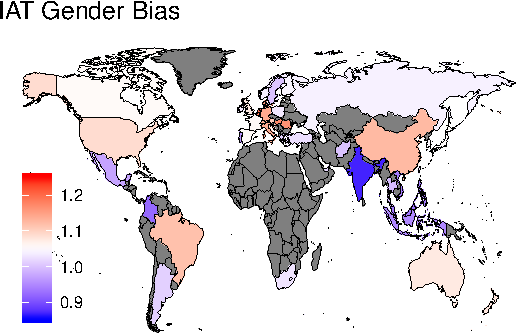
\includegraphics{figs/map-1} 

}

\caption[IAT gender bias effect size for 48 countries with available data]{IAT gender bias effect size for 48 countries with available data. All countries show a gender bias, with red indicating above average and blue indicating below average bias.}\label{fig:map}
\end{figure}
\end{CodeChunk}

We replicate two key findings in the literature on the gender-career IAT
(Nosek et al., 2002). First, participants overall showed a bias to
associate men with career and females with family (\emph{d} = 1.08).
Figure 1a shows the mean effect size for each of the 48 countries in our
sample, with participants from all countries showing a gender bias
(\emph{M} = 1.05; \emph{SD} = 0.07). Second, implicit and explicit bias
measures were moderately correlated both at the level of individual
participants (\emph{r} = 0.15; \emph{p} \textless{} .00001) and at the
level of countries (\emph{r} = 0.31; \emph{p} = 0.03).

\begin{CodeChunk}
\begin{figure}[t]

{\centering 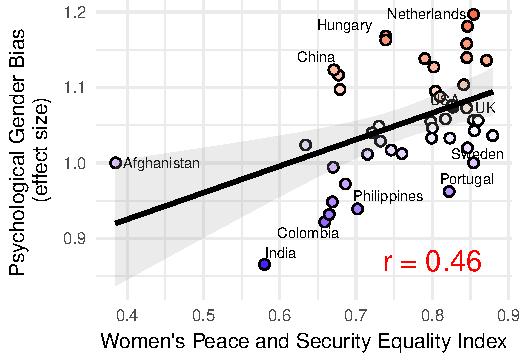
\includegraphics{figs/WPS_plot-1} 

}

\caption[Magnitude of the implicit gender bias (measured by the IAT) predicted by an independent measure of gender equality, Women's Peace and Security Index (WPS)]{Magnitude of the implicit gender bias (measured by the IAT) predicted by an independent measure of gender equality, Women's Peace and Security Index (WPS).  Each point corresponds to a country with notable points labeled. Contra our prediction, we find that countries with greater gender equality have larger gender implicit bias.[I'LL FIX THESE LABELS LATER]}\label{fig:WPS_plot}
\end{figure}
\end{CodeChunk}

Our independent measure of gender equality---the Women's Peace and
Security Index---was uncorrelated with explicit bias (\emph{r} = -0.01;
\emph{p} = 0.96). Counter to our expectations, we found that countries
such as the Netherlands, with allegedly greatest gender equality, have
participants with the highest implicit gender bias according to the IAT
(\emph{r} = 0.46; \emph{p} \textless{}.01; Fig.~1b).

\subsection{Discussion}\label{discussion}

In Study 1, we replicate previously reported patterns of gender bias in
the gender-career IAT literature, with roughly comparable effect sizes
(c.f.~Nosek, et al., 2002: overall effect: \emph{d} = .72;
explicit-implicit correlation: \emph{r} = .17; participant gender
effect: \emph{d} = .1). The weak correlation between explicit and
implicit measures is consistent with claims that these two measures tap
into different cognitive constructs (Oswald, Mitchell, Blanton, Jaccard,
\& Tetlock, 2013).

The novel finding from Study 1 is the direction of the correlation
between objective gender bias of a country (as measured by the WPS) and
implicit gender bias---participants in countries with greater gender
equality have \emph{greater} implicit gender bias. This robust
correlation is particularly surprising given that the English was likely
the second language for most of the participants in our sample, which
introduces additional noise into the measurement. In the General
Discussion, we speculate about possible reasons for this positive
correlation.

\section{Study 2: Gender bias and
semantics}\label{study-2-gender-bias-and-semantics}

In Study 2, we ask whether participants' psychological gender
biases---implicit and explicit---are correlated with the semantic
structure of their native languages. For example, are the semantics of
the words ``woman'' and ``family'' more similar in Hungarian than in
English? Both the language-as-reflection and language-as-causal
hypotheses predict a positive correlation between psychological and
semantic gender biases. Importantly, we expect psychological and
semantic gender biases to be correlated regardless of the direction of
the relationship between psychological and objective gender bias (WPS)
found in Study 1.

To model semantics, we turn to a machine-learning methods for deriving
lexical semantics from large corpora of text: auto-encoding neural
network models. The underlying assumption of these models is that the
meaning of a word can be described by the words it tends to co-occur
with---an approach known as distributional semantics (Firth, 1957).
Under this approach, a word like ``dog'' is represented as more similar
to ``hound'' than ``banana'' because it occurs with words more in common
with ``hound'' than ``banana'' where co-occurrences are effectively
defined at multiple hierarchical levels.

Recent developments in machine learning allow the idea of distributional
semantics to be implemented in a way that both takes into account many
features of local language structure while remaining computationally
tractable. The best known of these word embedding models is
\emph{word2vec} (Mikolov, Chen, Corrado, \& Dean, 2013). The model takes
as input a corpus of text and outputs a vector for each word
corresponding to its semantics. From these vectors, we can derive a
measure of the semantic similarity between two words by taking the
distance between their vectors (e.g., cosine distance). Similarity
measures estimated from these models have been shown to be highly
correlated with human judgements of word similarity (e.g., Hill,
Reichart, \& Korhonen, 2015), though more for some forms of similarity
than others (D. Chen, Peterson, \& Griffiths, 2017).

It turns out that various human biases as measured by the IAT can be
predicted from distributional semantics models like word2vec. Caliskan,
Bryson, and Narayanan (2017; henceforth \emph{CBN}) measured the
distance in vector space between the same sets of words that are
presented to participants in the IAT task. CBN found that these distance
measures are highly correlated with reaction times in the behavioral IAT
task. For example, in the career-gender IAT, CBN find a bias in the
semantics of English to associate males with career and females with
family, suggesting that the biases measured by the IAT are also found in
the lexical semantics of natural language.

In Study 2, we use the same method described by CBN to measure the
biases in the semantics of the natural languages spoken in the countries
of participants in Study 1. While CBN only analyzed biases for models
trained on English, we extend their method to compare biases across a
wide number of languages. To do this, we take advantage of a set of
models that have been pre-trained on a corpus of Wikipedia text in a
large number of languages (Bojanowski, Grave, Joulin, \& Mikolov, 2016).
In Study 2a, we replicate the CBN findings with the Wikipedia corpus; In
Study 2b, we show that the implicit gender biases reported in Study 1
for individual countries are correlated with the biases found in the
semantics of the natural language spoken by those participants.

\subsection{Study 2a: Replication of Caliskan, et
al.~(2017)}\label{study-2a-replication-of-caliskan-et-al.2017}

\subsubsection{Method}\label{method-1}

We use a word embedding model that has been pre-trained model on the
corpus of English Wikipedia using the fastText algorithm (Bojanowski et
al.,
2016)\footnote{Available here: https://github.com/facebookresearch/fastText/}.
The model contains 2,519,370 words with each word represented by a 300
dimensional vector.

Using the Wikipedia-trained model, we calculate an effect size for each
of the 10 biases reported in CBN which correspond to behavioral IAT
results existing in the literature:
flowers/insects--pleasant/unpleasant,
instruments/weapons--pleasant/unpleasant,
European-American/Afro-American--pleasant/unpleasant,\footnote{CBN test three versions of this bias.}
males/females--career/family, math/arts--male/female,
science/arts--male/female,
mental-disease/physical-disease--permanent/temporary, and
young/old--pleasant/unpleasant (labeled as WEAT 1-10 in CBN). We
calculate the bias using the same effect size metric described in CBN, a
standardized difference score of the relative similarity of the target
words to the target attributes (i.e.~relative similarity of male to
career vs.~relative similarity of female to career). This measure is
analogous the behavioral effect size measure in Study 1 and, like for
the behavioral effect size, larger values indicate larger gender bias.

\subsubsection{Results}\label{results-1}

\begin{CodeChunk}
\begin{figure}[t]

{\centering 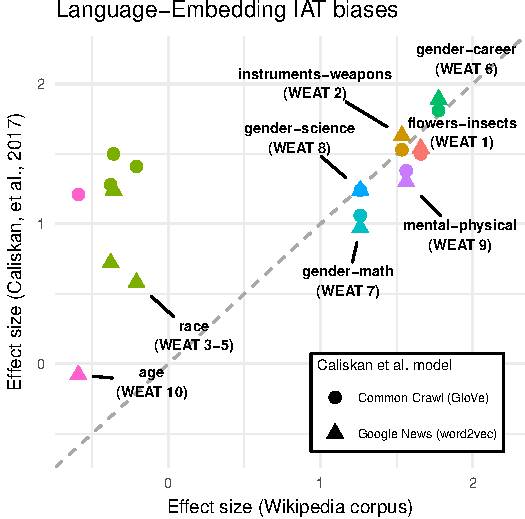
\includegraphics{figs/WEAT_plot-1} 

}

\caption[Effect sizes for the 10 IAT biases types (WEAT 1-10) reported in Caliskan et al]{Effect sizes for the 10 IAT biases types (WEAT 1-10) reported in Caliskan et al. (2017; CBN). The effect sizes reported in CBN are plotted against  effect sizes from the Wikipedia corpus.  Point color corresponds to  bias type, and point shape corresponds to the two CBN models trained on different corpora and with different algorithms.}\label{fig:WEAT_plot}
\end{figure}
\end{CodeChunk}

Figure 2 shows the effect size measures derived from the Wikipedia
corpus plotted against effect size estimates reported by CBN from two
different models (trained on the Common Crawl and Google News corpora).
With the exception of biases related to race and age, effect sizes from
the Wikipedia corpus are comparable to those reported by CBN. In
particular, for the gender-career IAT -- the bias relevant to our
current purposes -- we estimate the effect size to be 1.78, while CBN
estimates it as 1.81 (Common Crawl) and 1.89 (Google News).

\subsection{Study 2b: Cross-linguistic gender
semantics}\label{study-2b-cross-linguistic-gender-semantics}

With our corpus validated, we next turn toward examining the
relationship between psychological and linguistic gender biases. In
Study 2b, we estimate the magnitude of the gender-career bias in each of
the languages spoken in the countries described in Study 1 and compare
it with estimates of behavioral gender bias from Study 1. We predict
these two measures should be positively correlated.

\subsubsection{Method}\label{method-2}

\begin{CodeChunk}
\begin{figure}[t]

{\centering 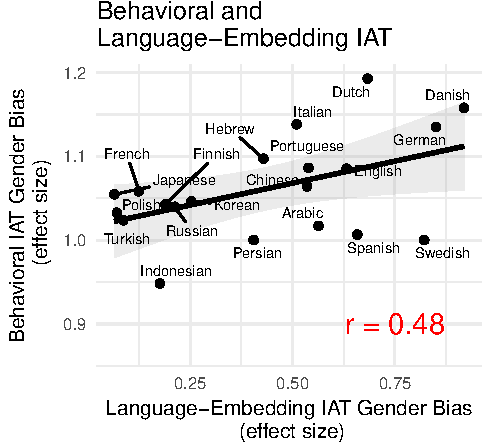
\includegraphics{figs/behavior_vs_language_plot-1} 

}

\caption[Gender bias effect size for each language from the behavioral IAT task (averaging across countries speaking the same primary language]{Gender bias effect size for each language from the behavioral IAT task (averaging across countries speaking the same primary language; Study 1) versus gender bias effect size estimated from embedding models trained on each language.}\label{fig:behavior_vs_language_plot}
\end{figure}
\end{CodeChunk}

For each country included in Study 1, we identified the most frequently
spoken language in those countries using the CIA factbook (Central
Intelligence Agency, 2017). This included a total of 31 unique
languages. For a sample of 20 of these languages (see Fig.~3), we had
native speakers translate the set of 32 words from the gender-career
IAT, with a slight
modification.\footnote{The language sample was determined by accessibility to native speakers, but included languages from a variety of language families.}
The original gender-career IAT task (Nosek et al., 2002) used proper
names to cue the male and female categories (e.g. ``John,'' ``Amy'').
Because there are not direct translation equivalents of proper names
across languages, we instead used a set of generic gendered words which
had been previously used for a different version of the gender IAT
(e.g., ``male,'' ``man,'' ``female,'' ``woman;'' Nosek et al., 2002).

We used these translations to calculate an effect size from the models
trained on Wikipedia in each language, using the same method as in Study
2a. We then compared the effect size of the linguistic gender bias to
the behavioral gender bias, averaging across countries that spoke the
same language and weighting by sample size.

\subsubsection{Results}\label{results-2}

Implicit IAT gender bias effect sizes were positively correlated with
effect sizes of gender bias estimated from the native language embedding
model (\emph{r} = 0.48; \emph{p} = 0.03; Fig.~3), suggesting that
countries that have more gender bias encoded in their language also have
a larger psychological gender bias. Explicit gender bias was not
reliably correlated with language gender bias (\emph{r} = 0.23; \emph{p}
= 0.33).

\section{Study 3: Gender bias and
grammar}\label{study-3-gender-bias-and-grammar}

Study 2 suggests that psychological gender bias and linguistic gender
bias are correlated, consistent with both the language-as-causal and
language-as-reflection hypotheses. In Study 3, we test the
language-as-causal hypothesis more directly by examining whether there
is a relationship between psychological gender bias and language along a
linguistic dimension that is unlikely to be a subject of rapid change --
namely, grammatical gender. While of course grammars do change, they are
less malleable than the semantics of words, and thus less likely to be
affected by psychological biases. We predict, therefore, that if
language causally influences psychological gender biases, languages that
encode gender grammatically will tend to have larger psychological
gender biases.

\subsection{Method}\label{method-3}

For each of the 31 languages represented in our sample of participants
(Study 1), we coded whether gender was encoded grammatically. We used a
coarse binary coding scheme, categorizing a language as encoding
grammatical gender if it made any gender distinction on noun classes
(male, female, common or neuter), and as not encoding gender
grammatically otherwise. We coded this distinction on the basis of the
WALS typological database (Feature 32a; Dryer \& Haspelmath, 2013) where
available, and consulted additional resources as necessary. Our sample
included 18 languages that encoded grammatical gender and 13 that did
not.

\subsection{Results}\label{results-3}

\begin{CodeChunk}
\begin{figure}[t]

{\centering 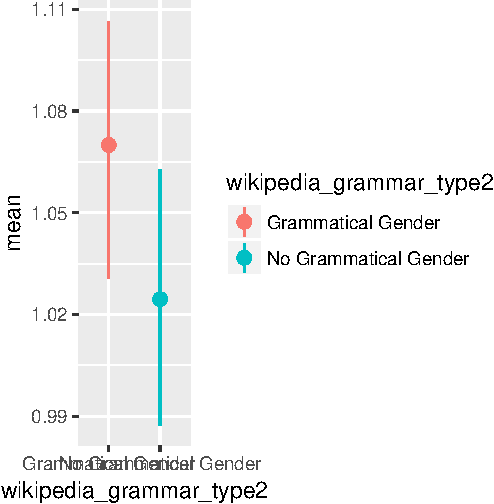
\includegraphics{figs/grammatical_gender_plot-1} 

}

\caption[Behavioral IAT effect size as a function of whether participants' (assumed) native language encodes gender grammatically]{Behavioral IAT effect size as a function of whether participants' (assumed) native language encodes gender grammatically. Each point corresponds to a language (N = 31) with outliers shown as triangles (jittered along the x-axis for visibility).}\label{fig:grammatical_gender_plot}
\end{figure}
\end{CodeChunk}

Languages that encode grammatical gender tended to have speakers with
greater psychological gender bias (Study 1; \emph{M} = 1.07; \emph{SD} =
0.08) compared to speakers of languages that do not grammatically encode
gender (\emph{M} = 1.02; \emph{SD} = 0.07), though this difference was
not reliable (\emph{d} = 0.69 {[}-0.08, 1.45{]}, \emph{t}(27.53) = 1.89;
\emph{p} = 0.07; Fig. 4). In a post-hoc analysis, we excluded outliers
located more than two standard deviations from the group mean (Hungarian
and Hindi). With these exclusions, we find a reliable difference between
language types (\emph{d} = 1.3 {[}0.46, 2.15{]}; \emph{t}(25.12) = 3.46;
\emph{p} \textless{} .01). In addition, we find the same pattern for
language IAT (Study 2), with languages that encode gender grammatically
tending to have larger language IAT gender biases, compared to those who
do not (\emph{t}(17.68) = 2.18; \emph{p} = 0.04). {[}INCLUDE REGRESSION
MODEL?{]}

\subsection{General Discussion}\label{general-discussion}

\section{Conclusion}\label{conclusion}

\section{References}\label{references}

\setlength{\parindent}{-0.1in} \setlength{\leftskip}{0.125in} \noindent

\hypertarget{refs}{}
\hypertarget{ref-bojanowski2016enriching}{}
Bojanowski, P., Grave, E., Joulin, A., \& Mikolov, T. (2016). Enriching
word vectors with subword information. \emph{arXiv Preprint
arXiv:1607.04606}.

\hypertarget{ref-boroditsky2001does}{}
Boroditsky, L. (2001). Does language shape thought?: Mandarin and
english speakers' conceptions of time. \emph{Cognitive Psychology},
\emph{43}(1), 1--22.

\hypertarget{ref-caliskan2017semantics}{}
Caliskan, A., Bryson, J. J., \& Narayanan, A. (2017). Semantics derived
automatically from language corpora contain human-like biases.
\emph{Science}, \emph{356}(6334), 183--186.

\hypertarget{ref-ciafactbook}{}
Central Intelligence Agency. (2017). The World Factbook. Retrieved from
\url{ttps://www.cia.gov/library/publications/the-world-factbook/index.html}

\hypertarget{ref-chen2017evaluating}{}
Chen, D., Peterson, J. C., \& Griffiths, T. L. (2017). Evaluating
vector-space models of analogy. \emph{arXiv Preprint arXiv:1705.04416}.

\hypertarget{ref-corbett1991}{}
Corbett, G. G. (1991). \emph{Gender}. Cambridge: Cambridge University
Press.

\hypertarget{ref-wals}{}
Dryer, M. S., \& Haspelmath, M. (Eds.). (2013). \emph{WALS online}.
Leipzig: Max Planck Institute for Evolutionary Anthropology. Retrieved
from \url{http://wals.info/}

\hypertarget{ref-fausey2010subtle}{}
Fausey, C. M., \& Boroditsky, L. (2010). Subtle linguistic cues
influence perceived blame and financial liability. \emph{Psychonomic
Bulletin \& Review}, \emph{17}(5), 644--650.

\hypertarget{ref-firth1957synopsis}{}
Firth, J. (1957). A synopsis of linguistic theory 1930-1955 in studies
in linguistic analysis, philological society. Oxford. reprinted in
Palmer, F.,(ed. 1968), Selected Papers of JR Firth, Longman, Harlow.

\hypertarget{ref-greenwald1998measuring}{}
Greenwald, A. G., McGhee, D. E., \& Schwartz, J. L. (1998). Measuring
individual differences in implicit cognition: The implicit association
test. \emph{Journal of Personality and Social Psychology}, \emph{74}(6),
1464.

\hypertarget{ref-greenwald2003understanding}{}
Greenwald, A. G., Nosek, B. A., \& Banaji, M. R. (2003). Understanding
and using the Implicit Association Test: An improved scoring algorithm.
\emph{Journal of Personality and Social Psychology}, \emph{85}(2), 197.

\hypertarget{ref-hill2015simlex}{}
Hill, F., Reichart, R., \& Korhonen, A. (2015). Simlex-999: Evaluating
semantic models with (genuine) similarity estimation.
\emph{Computational Linguistics}, \emph{41}(4), 665--695.

\hypertarget{ref-loftus1996eyewitness}{}
Loftus, E. F., \& Palmer, J. (1996). Eyewitness testimony. In
\emph{Introducing psychological research} (pp. 305--309). Springer.

\hypertarget{ref-master2012thinking}{}
Master, A., Markman, E. M., \& Dweck, C. S. (2012). Thinking in
categories or along a continuum: Consequences for children's social
judgments. \emph{Child Development}, \emph{83}(4), 1145--1163.

\hypertarget{ref-mikolov2013efficient}{}
Mikolov, T., Chen, K., Corrado, G., \& Dean, J. (2013). Efficient
estimation of word representations in vector space. \emph{arXiv Preprint
arXiv:1301.3781}.

\hypertarget{ref-nosek2002harvesting}{}
Nosek, B. A., Banaji, M. R., \& Greenwald, A. G. (2002). Harvesting
implicit group attitudes and beliefs from a demonstration web site.
\emph{Group Dynamics: Theory, Research, and Practice}, \emph{6}(1), 101.

\hypertarget{ref-oswald2013predicting}{}
Oswald, F. L., Mitchell, G., Blanton, H., Jaccard, J., \& Tetlock, P. E.
(2013). Predicting ethnic and racial discrimination: A meta-analysis of
iat criterion studies. \emph{Journal of Personality and Social
Psychology}, \emph{105}(2), 171.

\hypertarget{ref-phillips2003can}{}
Phillips, W., \& Boroditsky, L. (2003). Can quirks of grammar affect the
way you think? Grammatical gender and object concepts. In
\emph{Proceedings of the 25th annual meeting of the cognitive science
society} (pp. 928--933). Lawrence Erlbaum Associates Mahwah, NJ.

\hypertarget{ref-sera1994grammatical}{}
Sera, M. D., Berge, C. A., \& Castillo Pintado, J. del. (1994).
Grammatical and conceptual forces in the attribution of gender by
english and spanish speakers. \emph{Cognitive Development}, \emph{9}(3),
261--292.

\hypertarget{ref-tversky1981framing}{}
Tversky, A., \& Kahneman, D. (1981). The framing of decisions and the
psychology of choice. \emph{Science}, \emph{211}(4481), 453--458.

\hypertarget{ref-whorf1945grammatical}{}
Whorf, B. L. (1945). Grammatical categories. \emph{Language}, 1--11.

\hypertarget{ref-wps}{}
Women's Peace and Security Index. (2017). Retrieved from
\url{https://giwps.georgetown.edu/}

\end{document}
